\section{Teleoperated Manipulation Method}
	\label{sec:teleop_manip_method}
	
	Let us consider a humanoid robot equipped with a Laser Range Finder (LRF) placed at the head,
	as well as three cameras: at the head and at each hand.
	The LRF provides a point cloud of the environment, probably contaminated with noise due to the enviromental
	conditions of the disaster scenario; that is, even after a proper calibration it is not possible to consider
	that the 3D data precisely represents points belonging to objects in the environment, but within a certain
	amount of tolerance.
	On the other hand, the frame rate of the cameras, as well as the resolution, are intentionally set low
	foreseeing the effects of the degraded communication.
	
	This information of the environment, together with the sensorial information providing the current state of
	the robot, are the only information available to the operator, which has to supervise the robot while performing
	the tasks by establishing	high level goals, assisting with perception and changing parameters during the task.
	For this purpose, and under the circumstances stated above, we came up with a teleoperated manipulation method
	based on ``markers'' which assume minimum knowledge of the environment.
	This one is explained on the following.
	
	\subsection{Approaching to the target}
	
		The robot must achieve a proper stance with respect to the object(s) representing the target of the task,
		such that they be inside of the dextrous workspace of the hands of the robot.
		To do that the robot must perform a first measurement of the environment in order to check, together with the
		head camera, if the manipulation target is represented by some set of points of the resulting point cloud.
		In such a case, a preliminar alignment of a 3D object representing this manipulation target
		(the \emph{manipulation marker}) is first performed.
		
		By using the Graphical User Interface (GUI) provided by Choreonoid~\cite{Nakaoka_Choreonoid}, the Manipulation
		Marker is represented as the corresponding 3D model together with a set of arrows and rings which allow the
		operator to translate and rotate it with respect to its local reference frame,
		as depicted in \figurename~\ref{fig:ManipulationMarker}.
		
		\begin{figure}[b]
			\centering
			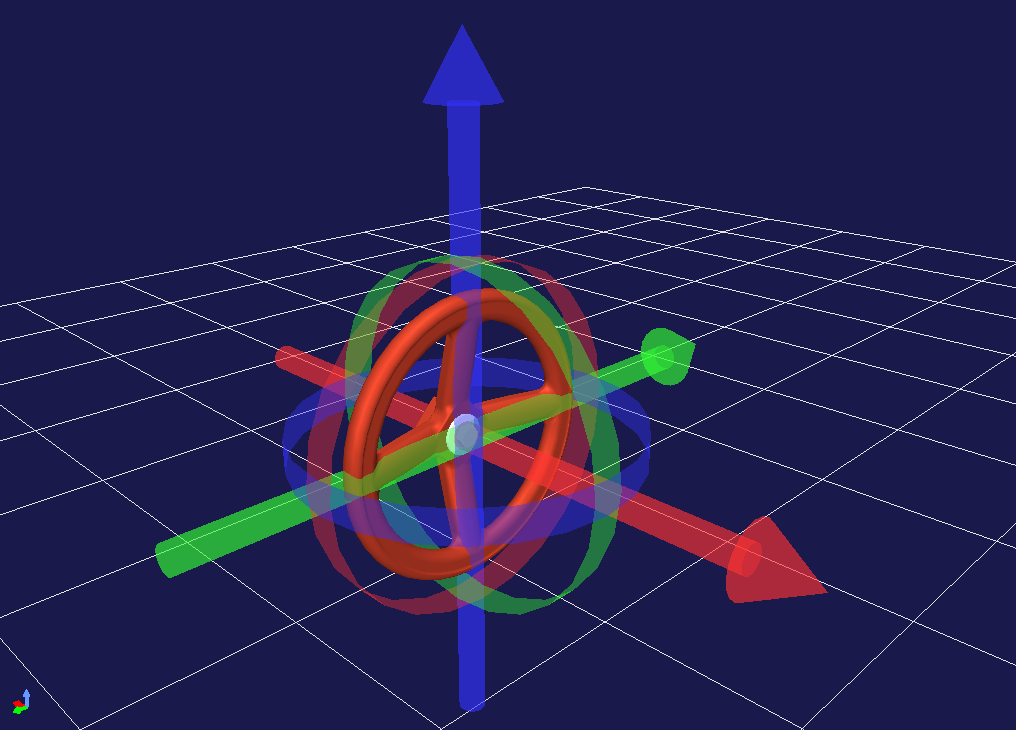
\includegraphics[height = 5.5cm]{img/ManipulationMarker}
			\caption{Manipulation Marker of a valve.}
			\label{fig:ManipulationMarker}
		\end{figure}

		Doing this alignment manually can be tedious, besides the fact that it may require a lot of time.
		To speed it up, it is possible to use a built in function included in the Point Cloud Library (PCL) that
		automatically alignes the marker with the best fit set of points, by providing maximum displacements,
		the number of iterations and some allowable error.
		However, ordinarily the robot will not be close enough to the object(s) for them to be measured with enough
		density of points, in such a way that the automatic alignment be prone to fail.
		One way to overcome this problem is to select one point of the point cloud belonging to the object and set
		this as the origin of the local reference frame of the Manipulation Marker, then the automatic alignment
		will lead to an alignment that may or may not require further small manual adjustments.
		
		One way to improve the initial alignment of the Manipulation Marker is to use beforehand information of the
		possible attitude of the object with respect to the nearest wall.
		For example, if the manipulation target is a box attached to the wall, its front face will probably be
		parallel to it.
		Knowing this, it is just the matter to identify the plane of the wall (and maybe the floor),
		get its mathematical representation and use it to define an initial attitude of the Manipulation Marker,
		requiring little automatic or manual adjustments.
		
		Once this is done, it is possible to define a proper stance of the robot (decided beforehand) with respect
		to the local reference frame of the Manipulation Marker.
		Then, by taking into account the height field of the floor (obtained from the point cloud) and avoiding the
		obstacles of the environment (walls and/or other objects), a proper footstep planning is performed in order
		for the humanoid robot to arrive to the desired stance~\cite{Morisawa}~\cite{Perrin}.
		
	\subsection{Grasping the target}
		
		Once humanoid the robot arrives to the desired stance, it has to perform another measurement.
		First, because of the positioning errors accumulated during its locomotion, and second,
		in order to obtain a more dense point cloud inteded for refining the alignment of the Manipulation Marker.
		
		Having done this refinement, it is possible to describe the attitude of the hands of the robot with respect
		to the local reference frame of the Manipulation Marker in order to approach to the manipulation target and
		grasp it, push it or pull it as required.
		Once decided, the whole-body Inverse Kinematics (IK) solution must be found, taking into account the redundancy
		of the robot to avoid collisions with the environment (represented with the point cloud)~\cite{Kanoun}.
		
		This relative attitude of the hands needs to be previously decided, such that the task be effectively carried
		out by means of smooth motions; that is, avoiding singular configurations and critical postures that may
		compromise the stability of the robot.
		However, these ones can be modified during the execution of the task if necessary, by means of a Hand Marker,
		a 3D representation of the hand and a set of arrows and rings which allow the operator to translate and rotate it
		with respect to its local reference frame, calculating at the same time the resulting configuration of the
		humanoid robot.
		See \figurename~\ref{fig:HandMarker}.
		
		\begin{figure}[b]
			\centering
			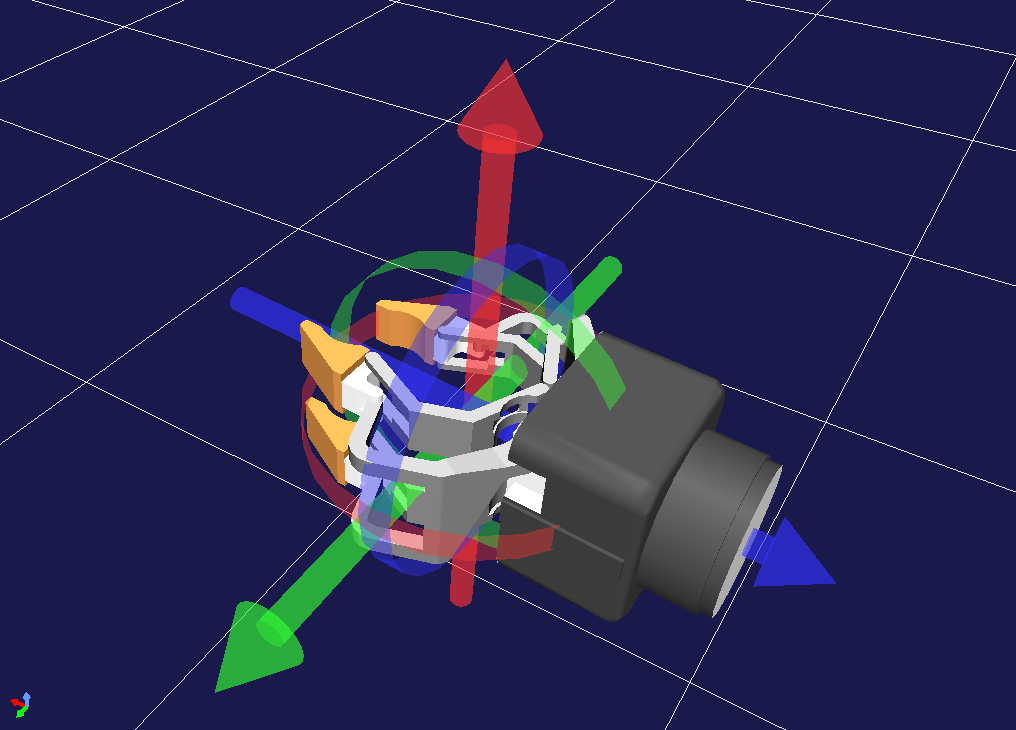
\includegraphics[height = 5.5cm]{img/HandMarker}
			\caption{Left Hand Marker.}
			\label{fig:HandMarker}
		\end{figure}
		
	\subsection{Dealing with uncertainties}
		\label{sub:uncertainties}
		
		Grasping the target with the desired relative attitude can be critical for some manipulation tasks,
		specifically if the target size is small when compared to the hand.
		However, it is worth to consider that the point cloud has an intrinsec noise, mainly caused as a result of the
		sunlight which complicates measurements.
		Then, it is not advisable to rely completely on the point cloud to plan the grasping motion,
		as the shown points may not represent actual points on the objects.
		
		One way to overcome this problem is to place the robot's hand within the view field of the LRF,
		and add some offset to the point cloud in order to match the corresponding points with the hand,
		whose attitude is known.
		This strategy practically improves the representation of the target objects by the point cloud but
		the precision may not be high enough.
		However, it can be used to approach to the manipulation targets (within some centimeters) before grasping them,
		with enough confidence that the hand is not going to collide unintentionally with the environment.
		
		Having done this, it is possible to use an approaching strategy in which the hand intentionally collides with
		the target by means of a slow motion, in order to use the force sensor installed in the hand to stop the hand
		when it senses a force greater than some established offset.
		Then, the real position of some plane of the target can be known relative to the hand, whose attitude can be
		computed by using forward kinematics and the actual joint values.
		The grasping point on the target can then be reached by moving the hand a very small distance with respect
		to its local reference frame.
		
	\subsection{Manipulating the target}
		
		Once the target is grasped, the relative attitude between the Manipulation Marker and the Hand Marker(s) can be
		set to be constant.
		Then, it is possible to manipulate the target by translating / rotating the Manipulation Marker, such that the
		required configuration of the humanoid robot be automatically calculated by means of solving the corresponding
		whole-body IK problem.
		In this way, a broad range of manipulation tasks can be accomplished by following this scheme, as illustrated
		by some examples which are described as follows.
		
		\begin{figure}[b]
			\centering
			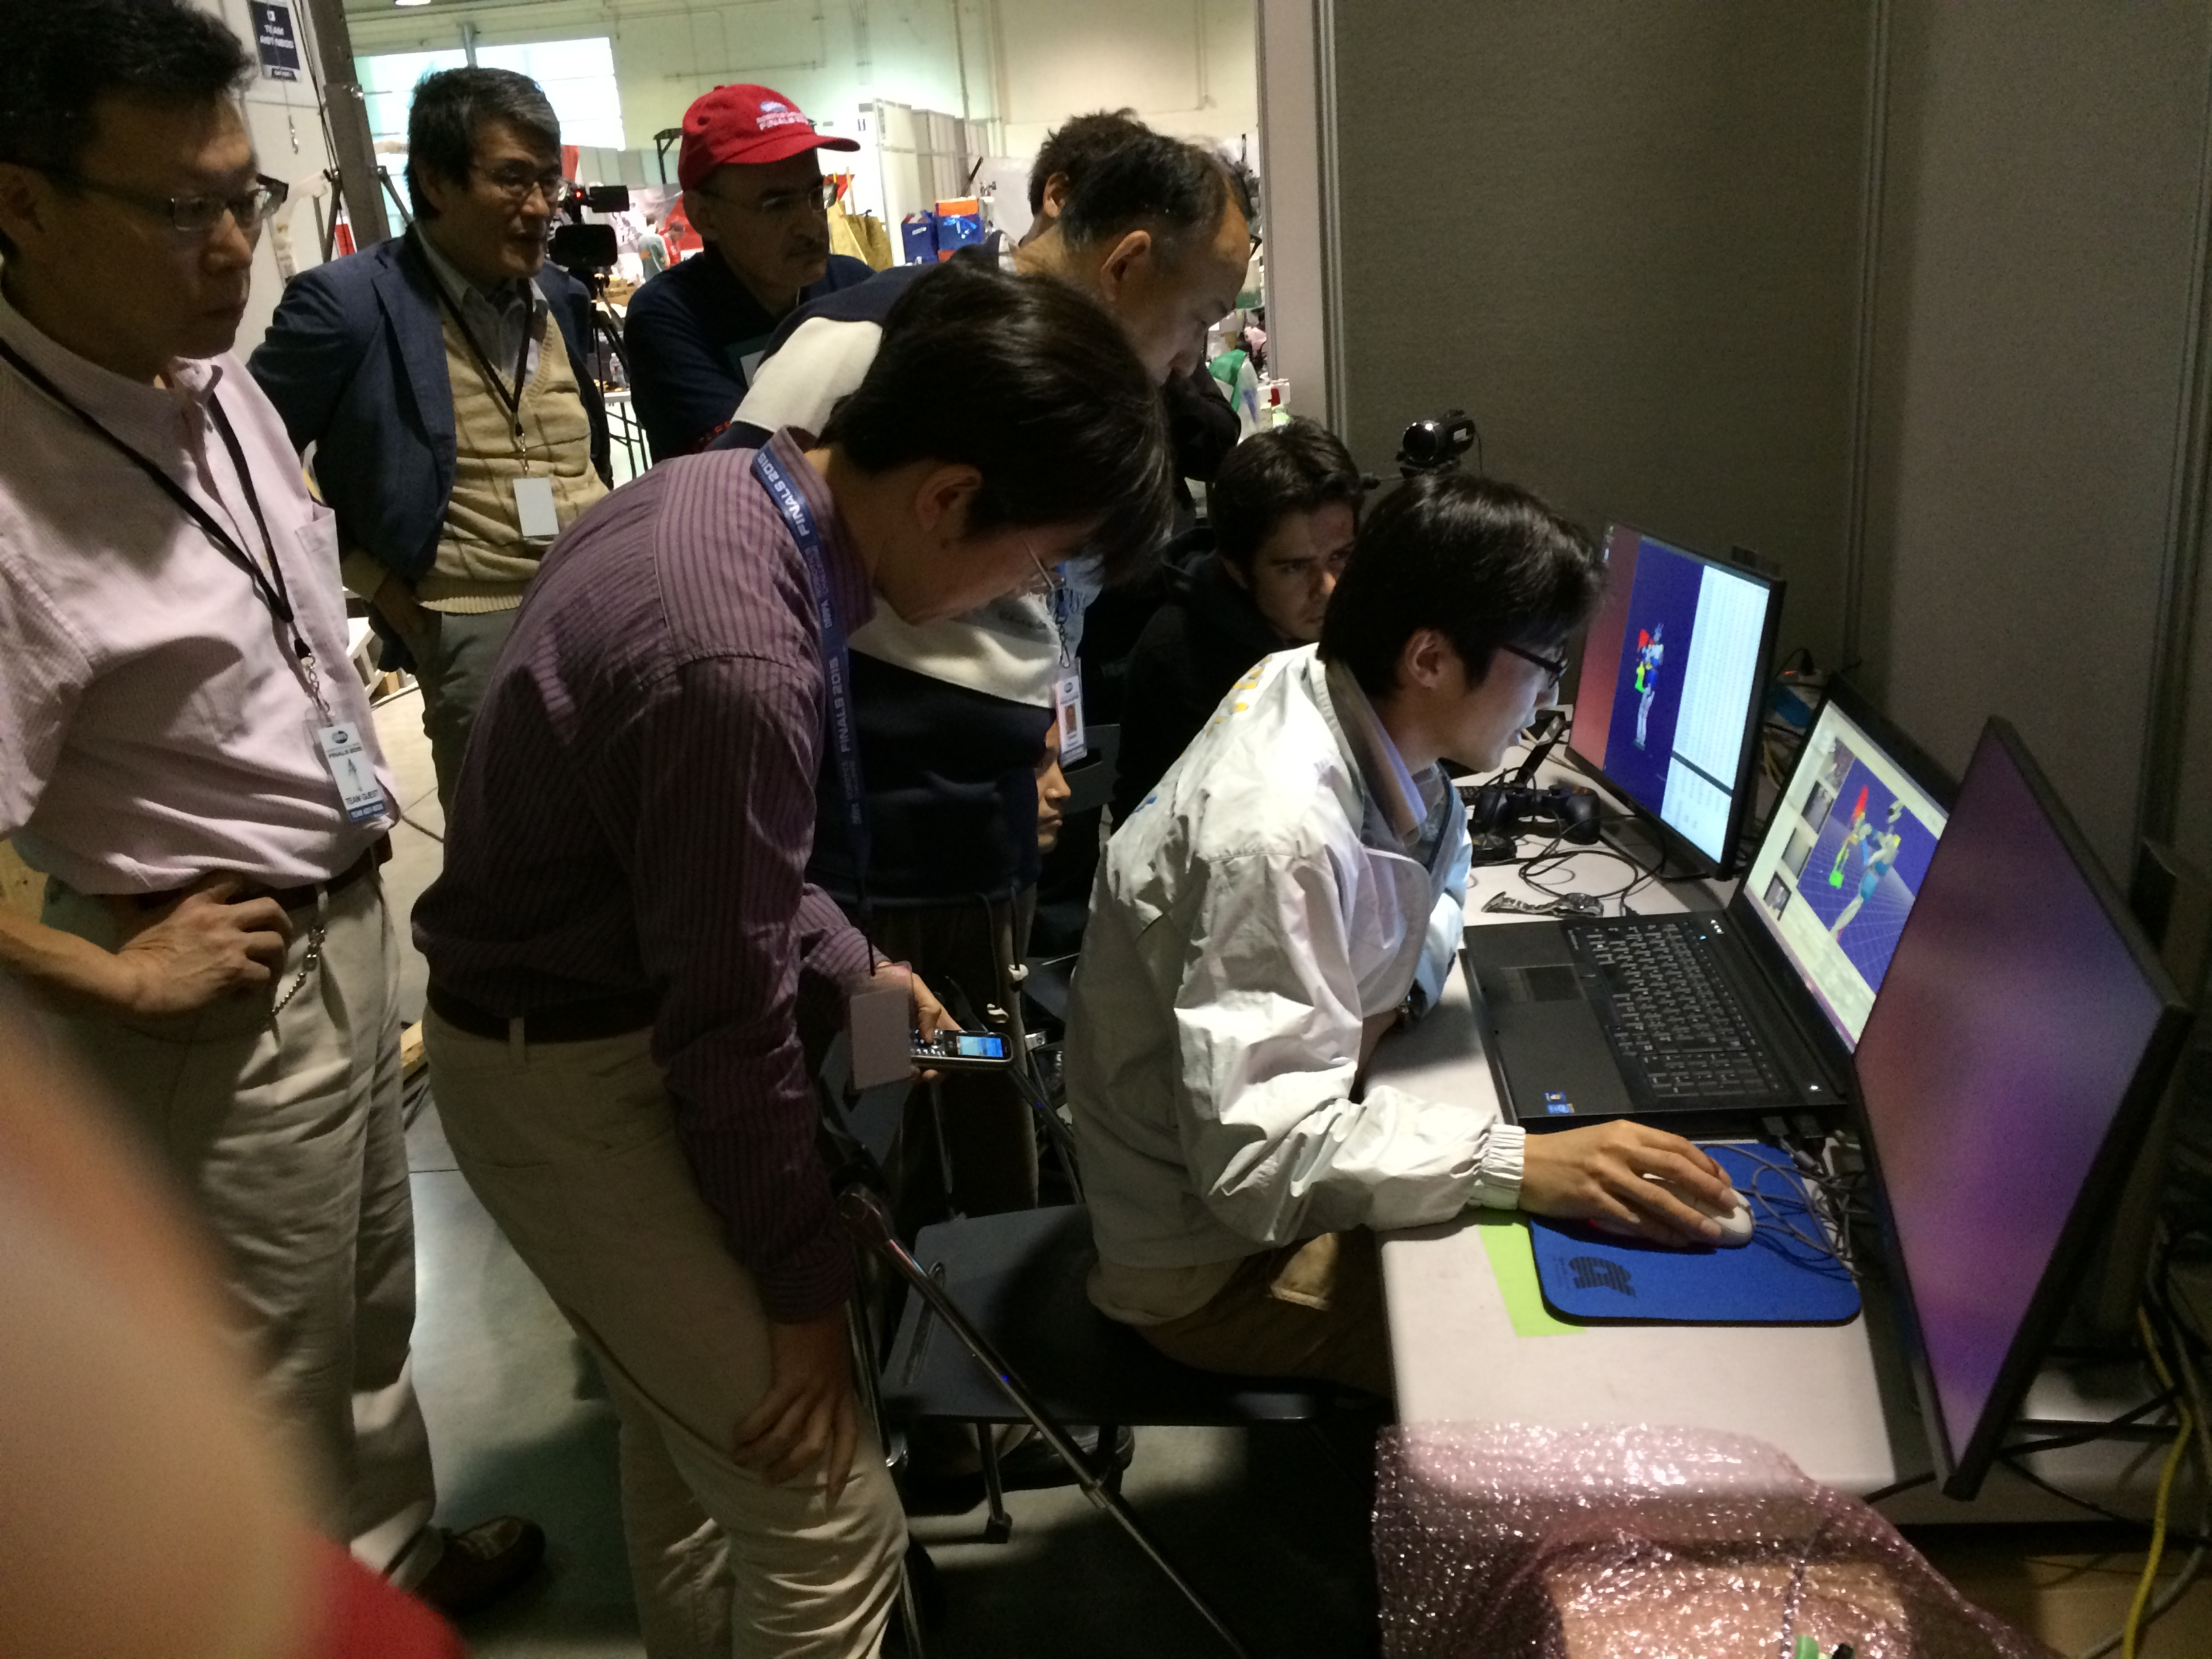
\includegraphics[height = 5.5cm]{img/OperationRoom}
			\caption{Operation Room.}
			\label{fig:OperationRoom}
		\end{figure}